\documentclass{beamer}
\usetheme{Madrid}
\usefonttheme{professionalfonts}
\usecolortheme{rose}
\usepackage{fontspec}
\setmainfont{Times New Roman}
\usepackage{amsmath}
\usepackage{enumitem}
\usepackage{bm}
\usepackage{booktabs}
\usepackage{tikz}
\usepackage{svg}
\usepackage{graphics}
\usepackage{appendixnumberbeamer}
\usepackage{mathtools}
\usepackage{subcaption}
\usepackage{comment}
\usepackage{slashed}
\usepackage[most]{tcolorbox}

\setlist[enumerate]{label=\arabic*.}
\setlist[itemize]{label=\textbullet}  % 标准 bullet 点
\tcbset{
  thickitembox/.style={
    colback=white,
    colframe=white,
    left=2mm,
    before skip=4pt,
    after skip=4pt,
    borderline west={3pt}{0pt}{gray},  % ← 这里控制线条粗细和颜色
    enhanced,
  }
}
\usetikzlibrary{decorations.pathreplacing}
\usetikzlibrary{arrows.meta}
\setlength{\parskip}{0.3em}
\newcommand{\aket}[1]{|#1\rangle}
\newcommand{\sket}[1]{|#1]}
\newcommand{\avg}[1]{\langle #1 \rangle}
\newcommand{\mdavg}[2]{\langle #1 \rangle\!\langle #2 \rangle}
\newcommand{\asqu}[1]{{\langle#1\rangle}^2}
\newcommand{\tif}[1]{\textit{\textbf{#1}}}
\AtBeginSection[]{
\begin{frame} 
    \frametitle{Contents}
    \tableofcontents[currentsection]
\end{frame}
}
\title[Application of BCFW]{\Large On-Shell Methods for Tree-Level Amplitudes in (De)Constructed Gauge Theory}
\author[Su Yingze]{
  \textbf{Su Yingze}\\[0.2em]
  \small Supervisor: \tif{Prof. Tanabashi Masaharu}
}

\institute[E Lab]{
  \normalsize Theoretical Elementary Particle Physics Laboratory\\[-0.3em]
  Nagoya University
}

\date[$11^{\text{th}}$ June]{June 11th, 2025}

\begin{document}
\setbeamertemplate{itemize item}{\normalsize\textbullet}
\begin{frame} % ← 不使用 [plain],保留 Madrid 顶部蓝条
  \titlepage
\end{frame}
\section{Motivation}
\begin{frame}{Why We Study Scattering Amplitudes?}
  \begin{enumerate}
    \item \textbf{Bridge between theory and experiment}
    \begin{itemize}
      \item Core prediction targets for high-energy collider experiments such as the LHC
      \item Any new theory (SUSY, GUTs, extra dimensions) must predict observable cross sections
    \end{itemize}
    \pause
    \item \textbf{Reveal deep structures of quantum field theory}
    \begin{itemize}
      \item Amplitudes exhibit hidden symmetries (e.g., dual conformal, Yangian) not visible in the Lagrangian
      \item These symmetries suggest deeper theoretical frameworks, such as amplituhedra or AdS/CFT correspondence
    \end{itemize}
  \end{enumerate}
\end{frame}


\begin{frame}
    \frametitle{Challenges we face befor}
\begin{center}
    
\tikzset{every picture/.style={line width=0.75pt}} %set default line width to 0.75pt        

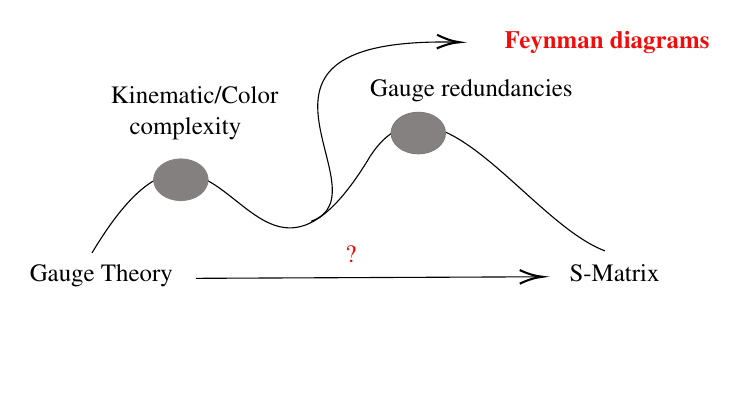
\begin{tikzpicture}[x=0.75pt,y=0.75pt,yscale=-1,xscale=1]
%uncomment if require: \path (0,300); %set diagram left start at 0, and has height of 300

%Curve Lines [id:da3663218891074064] 
\draw    (211.4,171.25) .. controls (275.46,64.25) and (285.26,224.75) .. (345.4,124.75) ;
%Shape: Ellipse [id:dp631421347808582] 
\draw  [color={rgb, 255:red, 134; green, 131; blue, 131 }  ,draw opacity=1 ][fill={rgb, 255:red, 133; green, 128; blue, 128 }  ,fill opacity=1 ] (241.14,136) .. controls (241.14,130.48) and (246.99,126) .. (254.21,126) .. controls (261.43,126) and (267.29,130.48) .. (267.29,136) .. controls (267.29,141.52) and (261.43,146) .. (254.21,146) .. controls (246.99,146) and (241.14,141.52) .. (241.14,136) -- cycle ;
%Curve Lines [id:da0018479507229188785] 
\draw    (345.4,124.75) .. controls (376.12,77.25) and (421.23,156.25) .. (458.49,170.25) ;
%Shape: Ellipse [id:dp37806345751603687] 
\draw  [color={rgb, 255:red, 128; green, 124; blue, 124 }  ,draw opacity=1 ][fill={rgb, 255:red, 133; green, 129; blue, 129 }  ,fill opacity=1 ] (355.53,113.5) .. controls (355.53,107.98) and (361.39,103.5) .. (368.61,103.5) .. controls (375.83,103.5) and (381.68,107.98) .. (381.68,113.5) .. controls (381.68,119.02) and (375.83,123.5) .. (368.61,123.5) .. controls (361.39,123.5) and (355.53,119.02) .. (355.53,113.5) -- cycle ;
%Straight Lines [id:da7438579232631651] 
\draw    (261.4,183.5) -- (426.42,182.76) ;
\draw [shift={(428.42,182.75)}, rotate = 179.74] [color={rgb, 255:red, 0; green, 0; blue, 0 }  ][line width=0.75]    (10.93,-3.29) .. controls (6.95,-1.4) and (3.31,-0.3) .. (0,0) .. controls (3.31,0.3) and (6.95,1.4) .. (10.93,3.29)   ;
%Curve Lines [id:da40606602539843883] 
\draw    (316.97,156) .. controls (355.02,142.32) and (265.25,67.01) .. (386.7,69.7) ;
\draw [shift={(388.54,69.75)}, rotate = 181.61] [color={rgb, 255:red, 0; green, 0; blue, 0 }  ][line width=0.75]    (10.93,-3.29) .. controls (6.95,-1.4) and (3.31,-0.3) .. (0,0) .. controls (3.31,0.3) and (6.95,1.4) .. (10.93,3.29)   ;

% Text Node
\draw (215.9,175.75) node [anchor=north] [inner sep=0.75pt]  [font=\small] [align=left] {{\fontfamily{ptm}\selectfont {\small  Gauge Theory}}\\{\fontfamily{ptm}\selectfont {\small  }}};
% Text Node
\draw (219.25,90) node [anchor=north west][inner sep=0.75pt]  [font=\small] [align=left] {{\small {\fontfamily{ptm}\selectfont Kinematic/Color}}\\{\small {\fontfamily{ptm}\selectfont  \ \ \ complexity}}};
% Text Node
\draw (344.1,86.5) node [anchor=north west][inner sep=0.75pt]  [font=\small] [align=left] {{\fontfamily{ptm}\selectfont {\small Gauge redundancies}}};
% Text Node
\draw (440.24,175.5) node [anchor=north west][inner sep=0.75pt]  [font=\small] [align=left] {{\fontfamily{ptm}\selectfont {\small S-Matrix}}};
% Text Node
\draw (332.23,166.5) node [anchor=north west][inner sep=0.75pt]  [font=\normalsize] [align=left] {{\fontfamily{ptm}\selectfont {\small \textcolor[rgb]{1,0,0}{?}}}};
% Text Node
\draw (408.97,63) node [anchor=north west][inner sep=0.75pt]  [font=\small] [align=left] {{\fontfamily{ptm}\selectfont {\small \textbf{\textcolor[rgb]{0.95,0.05,0.05}{Feynman diagrams}}}}};

\end{tikzpicture}
\end{center}
\vspace{-2.3em}
\begin{center}
\begin{tabular}{|c|c|c|c|c|c|c|c|}
\hline
$n=$ & 4 & 5 & 6 & 7 & 8 & 9 & 10 \\
\hline
     & 4 & 25 & 220 & 2485 & 34300 & 559405 & 10525900 \\
\hline
\end{tabular}
\end{center}
\pause

The answer is On-shell method.
    \begin{center}
        

\tikzset{every picture/.style={line width=0.75pt}} %set default line width to 0.75pt        

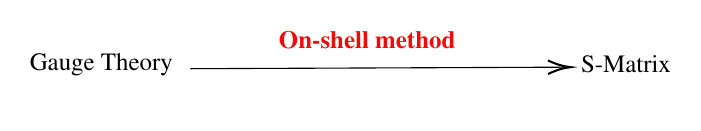
\begin{tikzpicture}[x=0.75pt,y=0.75pt,yscale=-1,xscale=1]
%uncomment if require: \path (0,300); %set diagram left start at 0, and has height of 300

%Straight Lines [id:da5445374886882226] 
\draw    (276.25,137) -- (457.5,136.26) ;
\draw [shift={(459.5,136.25)}, rotate = 179.77] [color={rgb, 255:red, 0; green, 0; blue, 0 }  ][line width=0.75]    (10.93,-3.29) .. controls (6.95,-1.4) and (3.31,-0.3) .. (0,0) .. controls (3.31,0.3) and (6.95,1.4) .. (10.93,3.29)   ;

% Text Node
\draw (233.4,128.25) node [anchor=north] [inner sep=0.75pt]  [font=\small] [align=left] {{\fontfamily{ptm}\selectfont {\small  Gauge Theory}}\\{\fontfamily{ptm}\selectfont {\small  }}};
% Text Node
\draw (463.24,129.5) node [anchor=north west][inner sep=0.75pt]  [font=\small] [align=left] {{\fontfamily{ptm}\selectfont {\small S-Matrix}}};
% Text Node
\draw (317.73,117.5) node [anchor=north west][inner sep=0.75pt]  [font=\normalsize] [align=left] {{\fontfamily{ptm}\selectfont {\small \textbf{\textcolor[rgb]{0.95,0.04,0.04}{On-shell method}}}}};


\end{tikzpicture}
\end{center}
\end{frame}
\section{Preliminary}
\begin{frame}
    \frametitle{Conventional VS. Modern}
    Usually, when we compute the gluon amplitudes by using Feynman diagram, we will obtain something like 
\begin{equation*}
    \begin{aligned}
&\mathcal{M}_s(p_1 p_2 \to p_3 p_4) = - \frac{g_s^2}{s} f^{abe} f^{cde} \\
&\quad \times \Big\{ 
-4\, \epsilon_1 \cdot \epsilon_3^* \, \epsilon_2 \cdot p_1 \, \epsilon_4^* \cdot p_3 
+ 2\, \epsilon_1 \cdot \epsilon_2 \, \epsilon_3^* \cdot p_1 \, \epsilon_4^* \cdot p_3 \\
&\quad - 2\, \epsilon_1 \cdot p_4 \, \epsilon_2 \cdot p_1 \, \epsilon_3^* \cdot \epsilon_4^*
+ \epsilon_1 \cdot \epsilon_2 \, p_4 \cdot p_1 \, \epsilon_3^* \cdot \epsilon_4^* \\
&\quad + 4\, \epsilon_1 \cdot \epsilon_4^* \, \epsilon_2 \cdot p_1 \, \epsilon_3^* \cdot p_4 
- 2\, \epsilon_1 \cdot \epsilon_2 \, \epsilon_3^* \cdot p_4 \, \epsilon_4^* \cdot p_1 \\
&\quad - 2\, \epsilon_1 \cdot p_2 \, \epsilon_2 \cdot p_3 \, \epsilon_3^* \cdot \epsilon_4^*
+ \epsilon_1 \cdot \epsilon_2 \, \epsilon_3^* \cdot \epsilon_4^* \, p_2 \cdot p_3 \\
&\quad + 4\, \epsilon_1 \cdot p_2 \, \epsilon_2 \cdot \epsilon_3^* \, \epsilon_4^* \cdot p_3 
- 2\, \epsilon_1 \cdot \epsilon_2 \, \epsilon_3^* \cdot p_2 \, \epsilon_4^* \cdot p_3 \\
&\quad + 2\, \epsilon_1 \cdot p_2 \, \epsilon_2 \cdot p_4 \, \epsilon_3^* \cdot \epsilon_4^* 
- \epsilon_1 \cdot \epsilon_2 \, \epsilon_3^* \cdot \epsilon_4^* \, p_4 \cdot p_2 \\
&\quad + 2\, \epsilon_1 \cdot p_3 \, \epsilon_2 \cdot p_1 \, \epsilon_3^* \cdot \epsilon_4^* 
- \epsilon_1 \cdot \epsilon_2 \, \epsilon_3^* \cdot \epsilon_4^* \, p_1 \cdot p_3 
\Big\}.
\end{aligned}
\end{equation*}
\end{frame}
\begin{frame}
    If you consider 5point case, it will become worser:
\begin{center}
    \textcolor{red}{$\bigstar$ There are nearly 10000 terms!}
\end{center}
\begin{columns}[T,onlytextwidth]
    % 左侧:传统图像
    \column{0.48\textwidth}
    \textbf{传统费曼图计算:}
    \begin{figure}
        \centering
        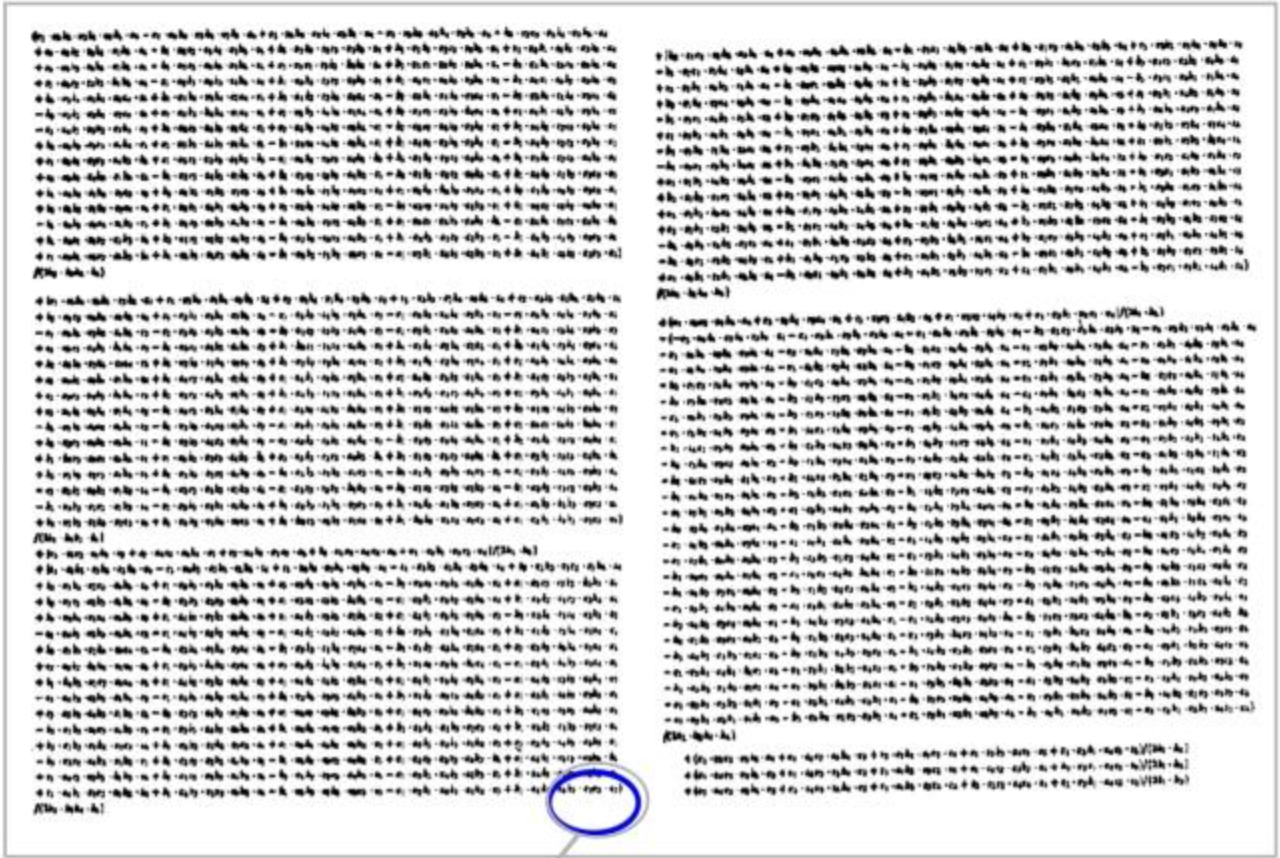
\includegraphics[width=\linewidth]{5pt.png}
    \end{figure}
    \pause 
    % 右侧:PT表达式
    \column{0.48\textwidth}
    \vspace{1.5em}
    \qquad \textbf{Parke–Taylor Formula:}
    \begin{gather*}
        \textcolor{red}{A_5(1^-,2^-,3^+,4^+,5^+)} =\\
        \textcolor{red}{\frac{\langle 1 2 \rangle^4}{\langle 1 2 \rangle \langle 2 3 \rangle \langle 3 4 \rangle \langle 4 5 \rangle \langle 5 1 \rangle}}
    \end{gather*}
\end{columns}
\vspace{2em}
\textcolor{red}{$\bigstar$ \Large It becomes quite simple and compact!}
\end{frame}
\begin{frame}
    \frametitle{Fantasitic result from Cauchy Theorem}
    %First, I will show the most important part in this report.
    \begin{block}{BCFW recursion relation}
        \begin{equation*}
            A_n=\sum_{\text{diagrams}\,I}\hat{A}_L(z_I)\frac{1}{P_I^2}\hat{A}_R(z_I)=\sum_{\text{diagrams}\,I}\raisebox{-1.3em}{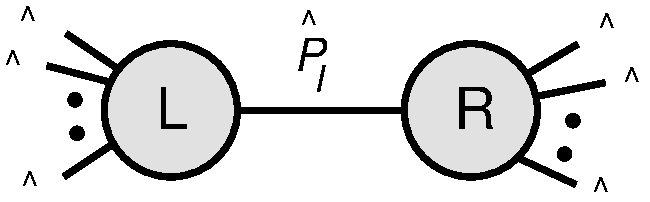
\includegraphics[height=3em]{recrel1.pdf}}
        \end{equation*}
    \end{block}
\vspace*{1em}
\pause
\tikzset{every picture/.style={line width=0.75pt}} %set default line width to 0.75pt        

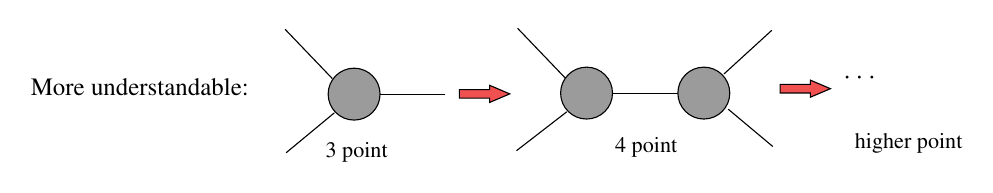
\begin{tikzpicture}[x=0.75pt,y=0.75pt,yscale=-1,xscale=1]
%uncomment if require: \path (0,300); %set diagram left start at 0, and has height of 300

%Shape: Circle [id:dp714548377068662] 
\draw  [fill={rgb, 255:red, 155; green, 155; blue, 155 }  ,fill opacity=1 ] (226.5,142.5) .. controls (226.5,135.6) and (232.1,130) .. (239,130) .. controls (245.9,130) and (251.5,135.6) .. (251.5,142.5) .. controls (251.5,149.4) and (245.9,155) .. (239,155) .. controls (232.1,155) and (226.5,149.4) .. (226.5,142.5) -- cycle ;
%Straight Lines [id:da2774899580018806] 
\draw    (205.75,111.25) -- (228.5,135) ;
%Straight Lines [id:da9722977180083648] 
\draw    (206.25,170.75) -- (229.5,151.5) ;
%Straight Lines [id:da6995788762725553] 
\draw    (283,142.5) -- (251.5,142.5) ;
%Shape: Circle [id:dp5472781658369114] 
\draw  [fill={rgb, 255:red, 155; green, 155; blue, 155 }  ,fill opacity=1 ] (338.5,142) .. controls (338.5,135.1) and (344.1,129.5) .. (351,129.5) .. controls (357.9,129.5) and (363.5,135.1) .. (363.5,142) .. controls (363.5,148.9) and (357.9,154.5) .. (351,154.5) .. controls (344.1,154.5) and (338.5,148.9) .. (338.5,142) -- cycle ;
%Straight Lines [id:da00014298672423462833] 
\draw    (317.75,110.75) -- (340.5,134.5) ;
%Straight Lines [id:da9890078833503395] 
\draw    (317.25,169.75) -- (341.5,151) ;
%Straight Lines [id:da6144558640267263] 
\draw    (395,142) -- (363.5,142) ;
%Right Arrow [id:dp2461212615941556] 
\draw  [fill={rgb, 255:red, 241; green, 80; blue, 80 }  ,fill opacity=1 ] (289.75,140.31) -- (304.3,140.31) -- (304.3,138.25) -- (314,142.38) -- (304.3,146.5) -- (304.3,144.44) -- (289.75,144.44) -- cycle ;
%Shape: Circle [id:dp17520461351076555] 
\draw  [fill={rgb, 255:red, 155; green, 155; blue, 155 }  ,fill opacity=1 ] (395,142) .. controls (395,135.1) and (400.6,129.5) .. (407.5,129.5) .. controls (414.4,129.5) and (420,135.1) .. (420,142) .. controls (420,148.9) and (414.4,154.5) .. (407.5,154.5) .. controls (400.6,154.5) and (395,148.9) .. (395,142) -- cycle ;
%Straight Lines [id:da6771243917531791] 
\draw    (417.25,132.75) -- (440.25,111.75) ;
%Straight Lines [id:da9753272478311303] 
\draw    (419.25,149.75) -- (440.75,167.75) ;
%Right Arrow [id:dp8085176402619464] 
\draw  [fill={rgb, 255:red, 241; green, 80; blue, 80 }  ,fill opacity=1 ] (444.25,137.81) -- (458.8,137.81) -- (458.8,135.75) -- (468.5,139.88) -- (458.8,144) -- (458.8,141.94) -- (444.25,141.94) -- cycle ;

% Text Node
\draw (82,133.5) node [anchor=north west][inner sep=0.75pt]   [align=left] {{\fontfamily{ptm}\selectfont {\small More understandable:}}};
% Text Node
\draw (473.5,130.9) node [anchor=north west][inner sep=0.75pt]    {$\cdots $};
% Text Node
\draw (224,164.5) node [anchor=north west][inner sep=0.75pt]   [align=left] {{\fontfamily{ptm}\selectfont {\footnotesize 3 point}}};
% Text Node
\draw (363.5,162) node [anchor=north west][inner sep=0.75pt]   [align=left] {{\fontfamily{ptm}\selectfont {\footnotesize 4 point}}};
% Text Node
\draw (479,160) node [anchor=north west][inner sep=0.75pt]   [align=left] {{\fontfamily{ptm}\selectfont {\footnotesize higher point}}};

\end{tikzpicture}

\vspace{1em}

\textcolor{red}{$\bigstar $ ~ From lower point to higher point!!}

\end{frame}
\begin{frame}{Spinor-Helicity Formalism}
\begin{block}{Helicity}
\textbf{Helicity} is defined as the projection of a particle's spin vector $\vec{S}$ onto the direction of its momentum $\vec{p}$:
\[
h = \frac{\vec{S} \cdot \vec{p}}{|\vec{p}|}
\]
\end{block}
\pause
% 文本说明(点击1出现)
\only<1->{
S-matrix is a function of momentum $p_i$ and helicity $h_i$
}

\vspace{0.8em}

% TikZ 图(点击1显示公式,点击2后补图形)
\begin{center}
\tikzset{every picture/.style={line width=0.75pt}}        
\begin{tikzpicture}[x=0.75pt,y=0.75pt,yscale=-1,xscale=1]

  % 点击1:显示公式
  \only<1>{
    \draw (260.25,137.9) node [anchor=north west][inner sep=0.75pt] 
          {$\mathcal{M}( p_{i} ,h_{i})$};
  }

  % 点击2及后:公式 + 圈箭头
  \only<2->{
    \draw (260.25,137.9) node [anchor=north west][inner sep=0.75pt] 
          {$\mathcal{M}( p_{i} ,\textcolor{red}{h_{i}})$};

    % 圆圈
    \draw  [color=red, draw opacity=1] 
      (302.8,146.93) .. controls (302.81,142.78) and (306.18,139.44) .. (310.32,139.45)
      .. controls (314.47,139.46) and (317.81,142.83) .. (317.8,146.97)
      .. controls (317.79,151.11) and (314.42,154.46) .. (310.28,154.45)
      .. controls (306.14,154.44) and (302.79,151.07) .. (302.8,146.93) -- cycle;

    % 箭头
    \draw [color=red, draw opacity=1] 
      (310.28,154.45) -- (296.03,178.04);
    \draw [shift={(295,179.75)}, rotate=301.13, color=red, draw opacity=1][line width=0.75pt] 
      (10.93,-3.29) .. controls (6.95,-1.4) and (3.31,-0.3) .. (0,0)
      .. controls (3.31,0.3) and (6.95,1.4) .. (10.93,3.29);

    % 注释文字
    \draw (173.25,181) node [anchor=north west][inner sep=0.75pt]  
      [font=\small,color=red,opacity=1] [align=left] 
      {How can we catch the information of helicity?};
  }

\end{tikzpicture}
\end{center}

% 点击3:Massless Case(用 uncover 保持排版稳定)
\uncover<3->{
\vspace{-1em}
\textbf{Massless Case:}
\begin{itemize}
  \item Momenta in spinor form:
    \[
      p_{\mu}\sigma^{\mu} = p_{\alpha\dot{\alpha}} = p_\alpha \tilde{p}_{\dot{\alpha}} = \aket{p}[p|
    \]
\end{itemize}
}

\end{frame}

\section{Model and Computation}

\begin{frame}{Introduction of quiver gauge theory}
\vspace{1em}
\begin{columns}[c]
    \column{0.43\textwidth}
    \centering
    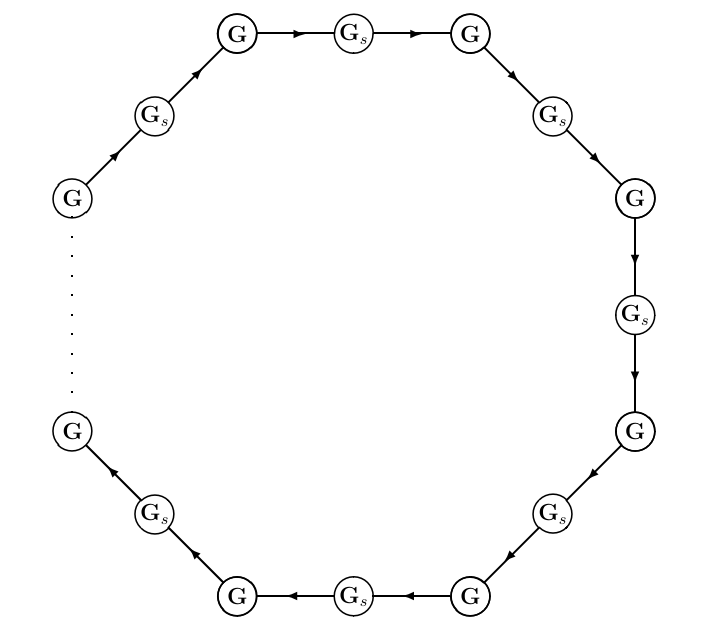
\includegraphics[width=100pt]{Moose.png}

    \column{0.14\textwidth}
    \centering
    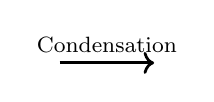
\begin{tikzpicture}[scale=0.8]
        \draw[->, line width=1pt] (0,0) -- (1.5,0)
            node[midway, above] {\footnotesize Condensation}; % ← 加文字
    \end{tikzpicture}

    \column{0.43\textwidth}
    \centering
    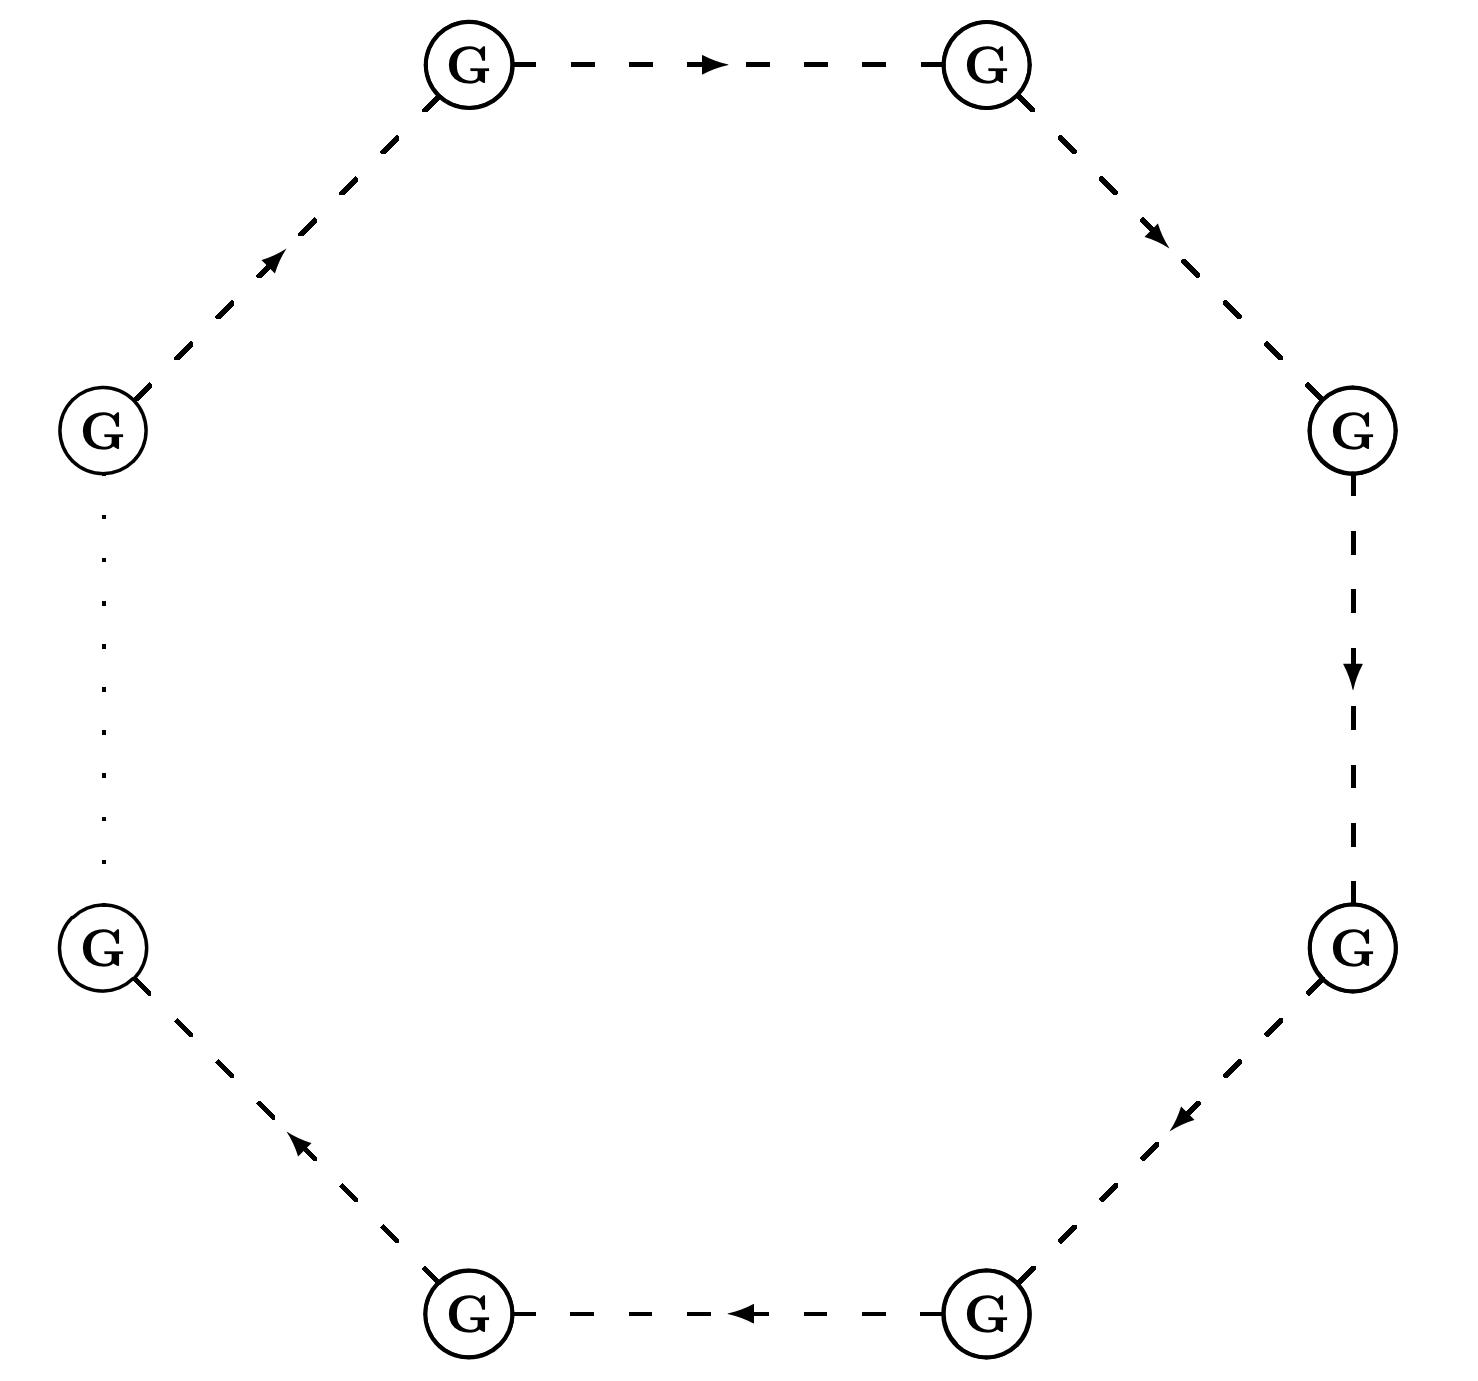
\includegraphics[width=100pt]{Moosed.jpeg}
\end{columns}


\pause
\raggedright
The Lagrangian can be written like
\begin{equation*}
    \mathcal{L} = -\sum_{i=1}^{N} \frac{1}{2} \mathrm{Tr}(F_i^2)
    + \sum_{i=1}^{N} \mathrm{Tr}\left[(D_\mu \Phi_i)^\dagger (D^\mu \Phi_i)\right],
\end{equation*}
here $F_i$ refers to the $i$th gauge field strength. The scalar field $\Phi_i$ transforms under the \textcolor{red}{bi-fundamental} representation, and the covariant derivative equals to
\begin{equation*}
    D_\mu \Phi_i = \partial_\mu \Phi_i - i g_i A_{i\mu} \Phi_i + i g_{i+1} \Phi_i A_{i+1\mu}.
\end{equation*}

\end{frame}

\begin{frame}
    It has been proposed that this model actually discretized a five-dimension gauge theory with gauge group $SU(m)$, where 
    only the fifth dimension are latticed. So it is an effective theory for 5d gauge theory.
     \vspace{1em} % 图与文字之间的间距
    \begin{center}
    \begin{minipage}{0.45\textwidth}
        \centering
        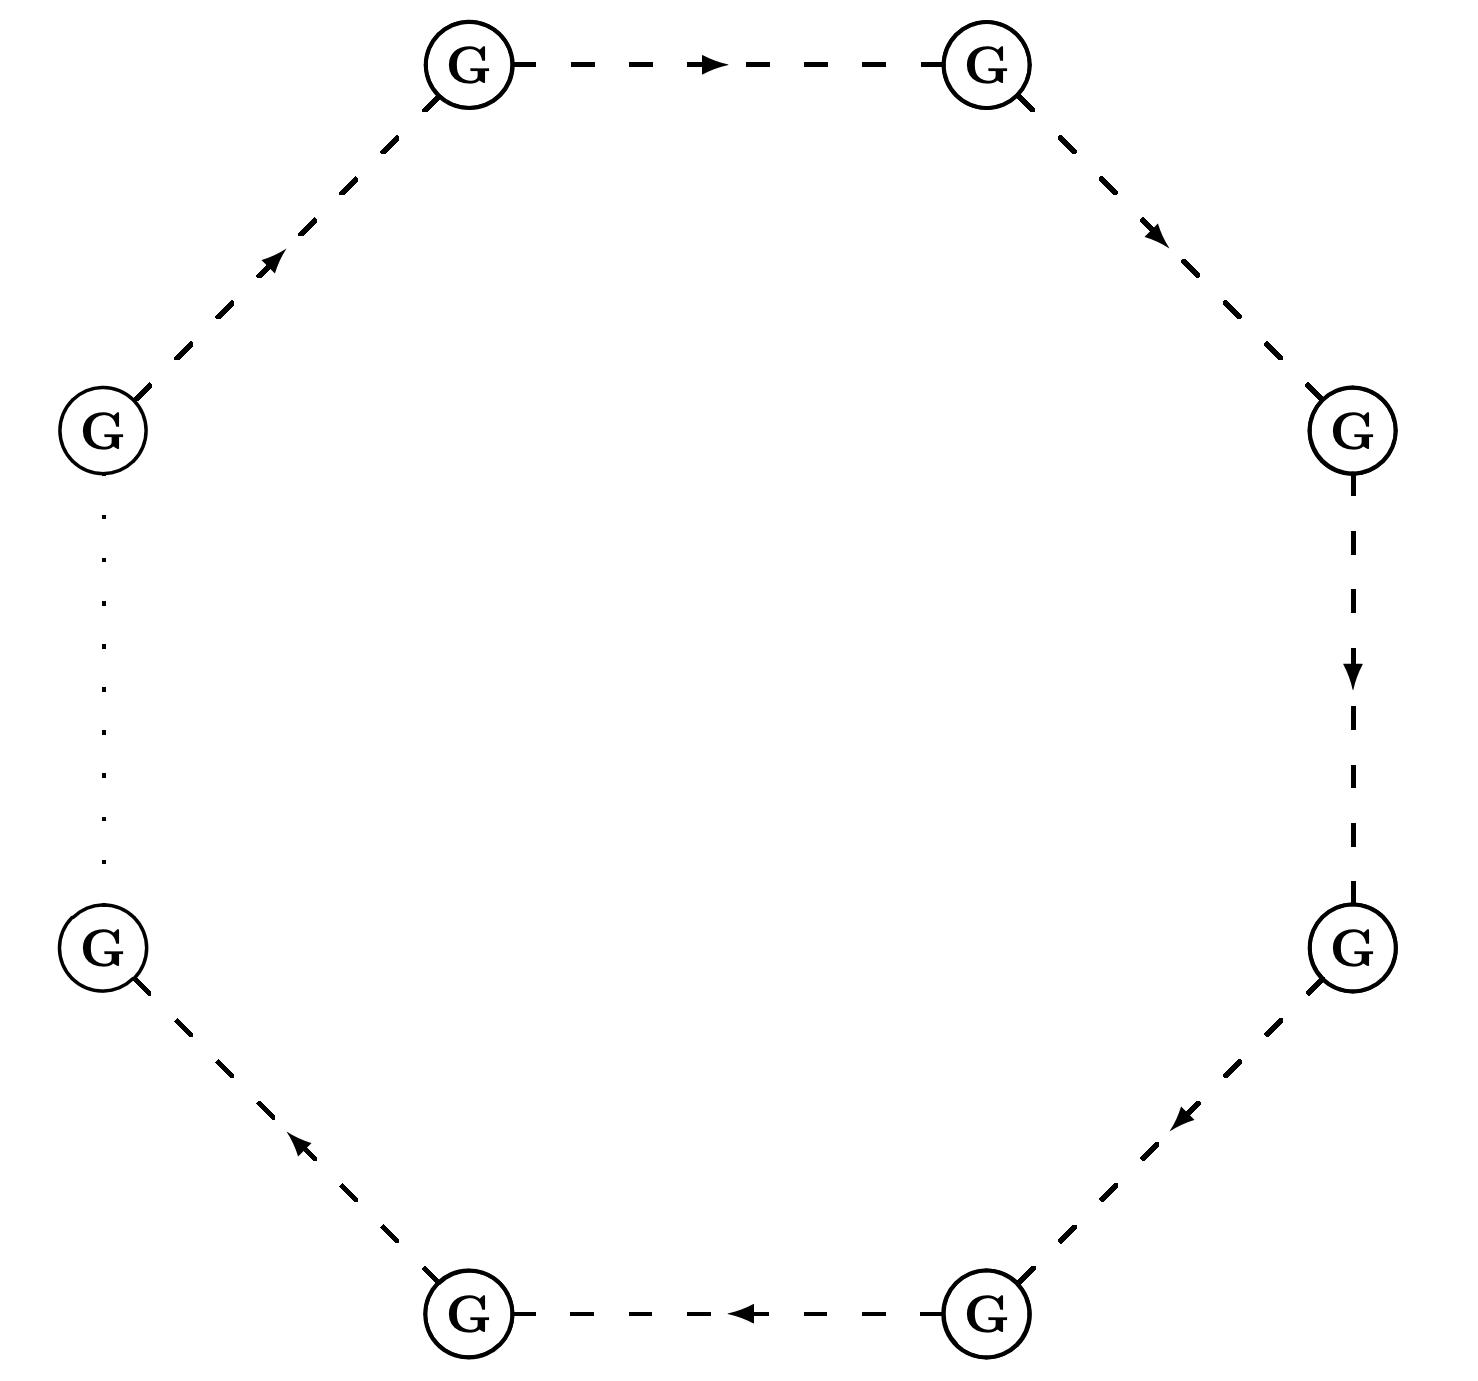
\includegraphics[width=0.6\linewidth]{Moosed.jpeg} % ← 替换为你的图片文件名
        \par\vspace{0.5em}
    \end{minipage}
    \hspace{0.05\textwidth}
    \begin{minipage}{0.45\textwidth}
        \centering
        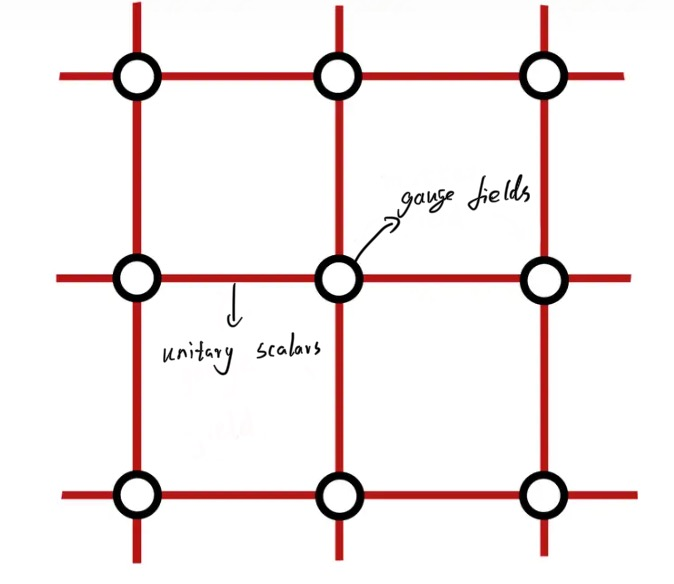
\includegraphics[width=0.6\linewidth]{Lattice.jpg} % ← 替换为你的图片文件名
        \par\vspace{0.5em}
    \end{minipage}
    \end{center}
    \pause
    After higgsing the scalar field, we can obtain a spectrum
    \begin{equation*}
        M_k^2=4g^2f_s^2\sin^2\left(\frac{\pi k}{N}\right)
    \end{equation*}
    This is precisely the \textcolor{red}{Kaluza-Klein} spectrum under $S^2$ compactification. 
\end{frame}
\begin{frame}
    \frametitle{Scattering Amplitudes from BCFW}
    For simplicity, we start from the two-site gauge theory with gauge fields $V_1$, $V_2$ and scalar fields $\Phi$, $\Phi^\dagger$.
    \begin{equation*}
        \mathcal{L}=-\frac{1}{2}\mathrm{Tr}(F_1)^2-\frac{1}{2}\mathrm{Tr}(F_2)^2+\mathrm{Tr}[(D_\mu\Phi)^\dagger(D^\mu\Phi)],
    \end{equation*}
We only foucus on the following amplitudes:
\begin{equation*}
    \textcolor{red}{nV_1,\qquad nV_2,\qquad\Phi^\dagger nV_1 \Phi,\qquad \Phi nV_2 \Phi^\dagger,\qquad \Phi^\dagger \Phi\Phi^\dagger \Phi}
\end{equation*}
here n can be any positive integer.
\end{frame}
\begin{frame}
    \frametitle{Basic building block -- 3-point}
    From the previous section, we have known that there are only two kinds of 3 point amplitude
    \begin{gather*}
        A[1,2,3^+]=\frac{[23][31]}{[12]},\qquad A[1,2,3^-]=\frac{\avg{23}\!\avg{31}}{\avg{12}}\\
        A[3^+,4^+,5^-]=\frac{[34]^3}{[45][53]},\qquad A[3^-,4^-,5^+]=\frac{\avg{34}^3}{\avg{45}\!\avg{53}}
    \end{gather*}
    By using the 3 point building block, we can construct 4 point color-ordered amplitudes from BCFW recursion relation.
\end{frame}
\begin{frame}
    \frametitle{Gauge boson sector}
    \begin{itemize}
        \item n$ V_1$ or n$V_2$\\
        This part is completely the same as the pure gluon amplitude, so we can directly borrow the
        existing results.
        \begin{equation*}
            \boxed{\text{Parke - Talyor Formula}:\quad A[\cdots,i^-,\cdots,j^-,\cdots]=\frac{\avg{ij}^4}{\avg{12}\!\avg{23}\cdots\avg{n1}}}
        \end{equation*}
        \textcolor{red}{Notice that this formula only applies to MHV amplitudes, although the NMHV can be completely solved.}
    \end{itemize}
\end{frame}

\begin{frame}
    \frametitle{SQCD like sector}
    \begin{itemize}
        \item $\Phi^\dagger V_1V_1\Phi$\\
        Here we compute the color-ordered amplitude $A[1,2,3^+,4^-]$. We choose $[2,3\rangle$ shift
        \begin{gather*}
        \hat{\sket{2}}=\sket{2}-z\sket{3},\qquad \hat{\aket{2}}=\aket{2} \\
        \hat{\sket{3}}=\sket{3},\qquad \hat{\aket{3}}=\aket{3}+z\aket{2}
        \end{gather*}
        The amplitudes can be computed 
        \begin{align*}
            A[1,2,3^+,4^-]=(-1)\frac{\avg{14}^2\avg{24}^2}{\mdavg{12}{23}\!\mdavg{34}{41}}
        \end{align*}
        \item $\Phi^\dagger V_1V_1V_1\Phi$
            \begin{equation*}
                A[1,2,3^+,4^+,5^-]=\frac{\avg{15}^2\!\avg{25}^2}{\mdavg{12}{23}\!\mdavg{34}{45}\!\avg{51}}
            \end{equation*}
    \end{itemize}
\end{frame}

\begin{frame}
    \begin{itemize}
        \item $\Phi^\dagger (nV_1)\Phi$
            \begin{equation*}
                A[1,2,\cdots,(n+2)^-]=(-1)^{n+1}\frac{\avg{1,n+2}^2\avg{2,n+2}^2}{\mdavg{12}{23}\cdots\mdavg{n+1,n+2}{n+2,1}}
            \end{equation*}
            \textcolor{red}{$\star$ Bonus relation: \begin{equation*}
                A[1,2,3^+,4^+]=0\quad \Rightarrow  \quad A[1,2,3^+,\cdots,n^+]=0 \end{equation*}}
        For the amplitude $\Phi (nV_2)\Phi^\dagger$, we can obtain nearly the same expression.
    \end{itemize}
\end{frame}

\begin{frame}
    \frametitle{Pure 2-site amplitude}
    \begin{itemize}
        \item $\Phi V_2 \Phi^\dagger V_1$
        \begin{equation*}
            A[1,2,3_1^+,4_2^-]=\frac{\mdavg{14}{24}}{\mdavg{13}{23}}
        \end{equation*}
        \item $\Phi V_2 \Phi^\dagger V_1V_1$
        \begin{equation*}
            A[1,2,3_1^+,4_1^+,5_2^-]=(-1)\frac{\avg{2\textcolor{green}{5}}^2\!\avg{1\textcolor{green}{5}}^2}{\textcolor{blue}{\mdavg{23}{34}\!\avg{41}}\textcolor{red}{\mdavg{25}{51}}}
        \end{equation*}
        \item $\Phi V_2V_2 \Phi^\dagger V_1V_1$
        \begin{equation*}
            A[1,2,3_1^+,4_1^+,5_2^+,6_2^-]=\frac{\avg{2\textcolor{green}{6}}^2\!\avg{1\textcolor{green}{6}}^2}{\textcolor{blue}{\mdavg{23}{34}\!\avg{41}}\!\textcolor{red}{\mdavg{25}{56}\!\avg{61}}}
        \end{equation*}       
    \end{itemize}
\end{frame}

\begin{frame}
    \begin{itemize}
        \item Compact formula for general case
        \begin{equation*}
            A=\frac{\asqu{2\textcolor{green}{a}}\!\asqu{1\textcolor{green}{a}}}{\underbrace{\avg{2\textcolor{blue}{\star}}\cdots \avg{\textcolor{blue}{\star}1}}_{SU(N_1)}\underbrace{\avg{2\textcolor{red}{\ast} }\cdots \avg{\textcolor{red}{\ast} 1}}_{SU(N_2)}}
        \end{equation*} 
        \begin{minipage}{0.7\textwidth}
            \raggedright  % 或者 \centering 或 \raggedleft
            \textcolor{green}{Green:} \,Particle with $-$ helicity\\
            \textcolor{blue}{Blue:}\, Particle belongs to the first gauge group\\
            \textcolor{red}{Red:}\, Particle belongs to the second gauge group\\
            $\star$: \,Order for gauge group 1\\
            $\ast$: \,Order for gauge group 2 
            \end{minipage}
       
    \end{itemize}
\end{frame}
\section{Summary}
\begin{frame}
    \frametitle{Summary}
    \begin{itemize}
        \item Introduce the on-shell method, including BCFW recursion relation, spinor-helicity formalism, etc.
        \item Introduce a (de)constructed gauge theory model, which is an effective field theory for 5 dimension gauge theory.
        \item Much of the scattering amplitudes in this model can be recursively computed by BCFW, and some compact formulas are offered.
    \end{itemize}
\end{frame}
\begin{frame}
    \centering
    \Huge Thanks for your attention!
\end{frame} 
\appendix

\begin{frame}
    
    \textbf{Brief explaination}: We choose two momentum to be shifted oppositely 
    \begin{equation*}
        p_i\rightarrow\hat{p}_i(z)\equiv p_i-zk,\qquad p_j\rightarrow\hat{p}_j(z)\equiv p_j+zk
    \end{equation*}
    satisfying 
    \begin{equation*}
        k^2=0,\qquad p_i\cdot k=0,\qquad p_j\cdot k=0
    \end{equation*}
    
    We consider amplitude $A_n$ in terms of shifted momentum $\hat{p}_i^\mu$ instead of original real momentum. 
    \begin{equation*}
        A_n \longrightarrow \hat{A}_n(z)
    \end{equation*}
    \pause
    If we consider the meromorphic function $\frac{\hat{A}_n(z)}{z}$ in the complex plane.
    From Cauchy Theorem, we can ontain
    \begin{equation*}
        A_n=-\sum_{z_I}\textrm{Res}|_{z=z_I}\frac{\hat{A}_n(z)}{z}+B_n,
    \end{equation*}
    where $B_n$ is the residue of the pole at $z=\infty$, called boundary term.
\end{frame}
\begin{frame}
   
    \vspace{-1em}
    \begin{figure}[htbp]
        \centering
        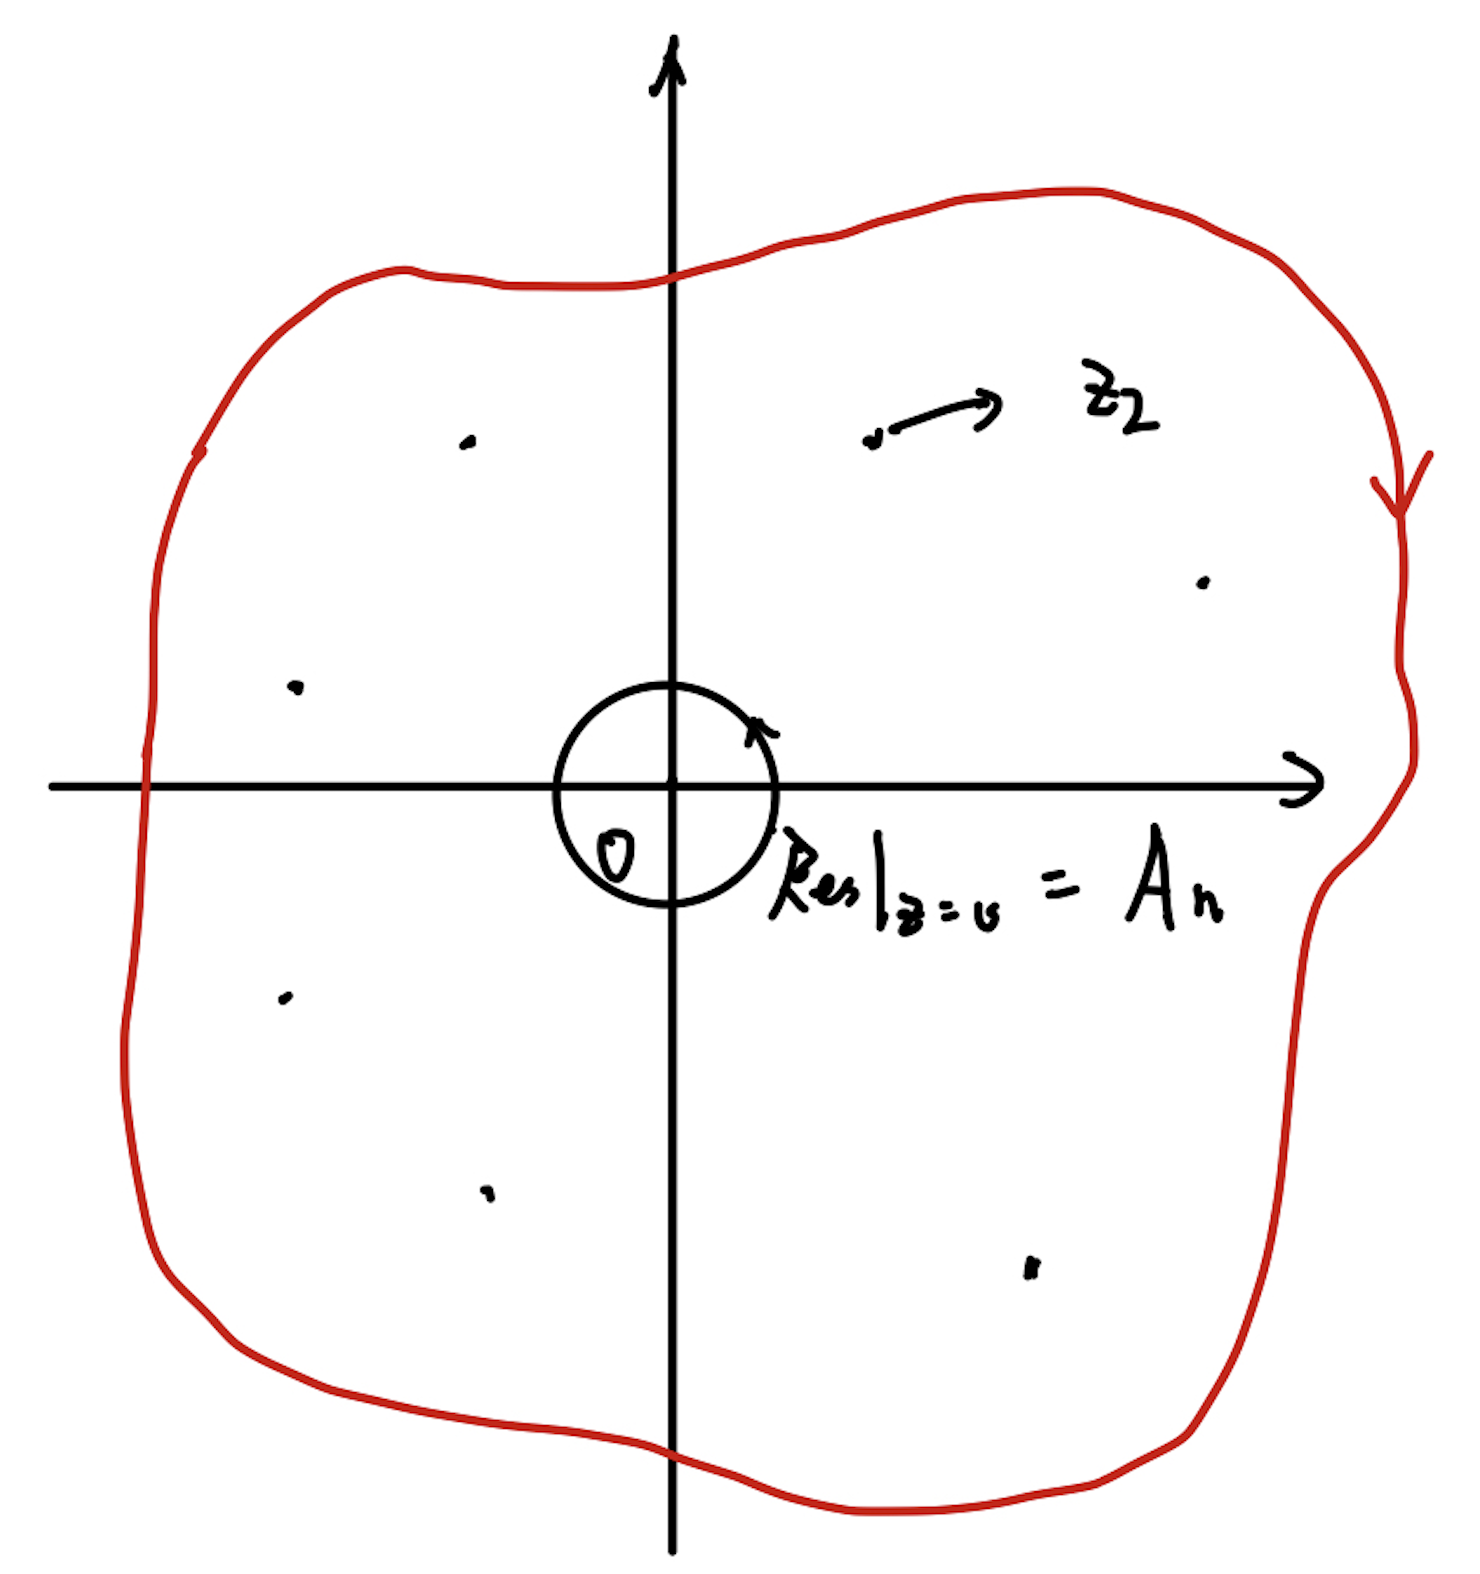
\includegraphics[width=0.3\textwidth]{CT.png}
    \end{figure}
    \vspace{-1.5em}
    %Then, at a $z_I$ pole, the propagator $\hat{P}_I^2$ goes to on-shell. In that limit, the shifted amplitude
    %\textcolor{red}{factorizes} into to on-shell parts (Unitarity)
   \textcolor{red}{$\bigstar$ The most important point here is that}
    \begin{equation*}
        \boxed{\color{red}\mathrm{Res}|_{z=0}\frac{\hat{A}_n(z)}{z}=\hat{A}_n(0)=A_n}
    \end{equation*}
    and 
\begin{equation*}
    \mathrm{Res}|_{z=z_I}=\hat{A}_L(z_I)\frac{1}{P_I^2}\hat{A}_R(z_I)
\end{equation*}
\end{frame}

\begin{frame}
    \frametitle{Large z behavior}
    In the BCFW formula, the boundary term $B_n$ affects a lot
    \begin{equation*}
        A_n=-\sum_{z_I}\mathrm{Res}|_{z=z_I}\frac{\hat{A}_n(z)}{z}+B_n,
    \end{equation*}
    In most applications. one assumes or much better, proves $B_n=0$. This is often justified by declaring a stronger condition
    \begin{equation*}
        \textcolor{red}{\hat{A}_n(z)\rightarrow 0 \quad \text{for} \quad z\rightarrow \infty} 
    \end{equation*}
    Here I show the large z behavior for gluon scattering 
    \begin{center}
        \begin{tabular}{lrc}
            \toprule
            $[i\, \textbackslash \, j\rangle $ & $+$ & $-$ \\
            \midrule
            $+$ & $1/z$ & $z^3$ \\
            $-$ & $1/z$ & $1/z$ \\
            \bottomrule
          \end{tabular}
    \end{center}
\end{frame}

\begin{frame}
    \frametitle{ On-shell 3-point can be completely determined}
    For the complex momentum, we have 
    \begin{equation*}
        \aket{1}\propto \aket{2}\propto \aket{3} \qquad or \qquad \sket{1}\propto \sket{2}\propto \sket{3}
    \end{equation*}
    \[
    \boxed{
    \begin{aligned}
        A_3^{h_1h_2h_3} &= c\avg{12}^{h_3-h_1-h_2}\avg{31}^{h_2-h_1-h_3}\avg{23}^{h_1-h_2-h_3}
        \quad & h_1+h_2+h_3 < 0 \\[0.5em]
        A_3^{h_1h_2h_3} &= c' [12]^{h_1+h_2-h_3}[23]^{h_2+h_3-h_1}[31]^{h_3+h_1-h_2}
        \quad & h_1+h_2+h_3 > 0
    \end{aligned}
        }
    \]

    \textbf{\textcolor{red}{$\star$\,All massless on-shell 3-point ampltides are completely determined by little group scaling!}}
    
    \textbf{Example}: 3-gluon amplitude\\
    \begin{equation*}
        A_3(g_1^-,g_2^-,g_3^+)=g\frac{\avg{12}^3}{\avg{23}\!\avg{31}}
    \end{equation*}
\end{frame}
\end{document}